\documentclass[tikz]{standalone}
\usepackage[american]{circuitikz}
\usepackage{pgfplots}
\pgfplotsset{compat=1.18}
\begin{document}
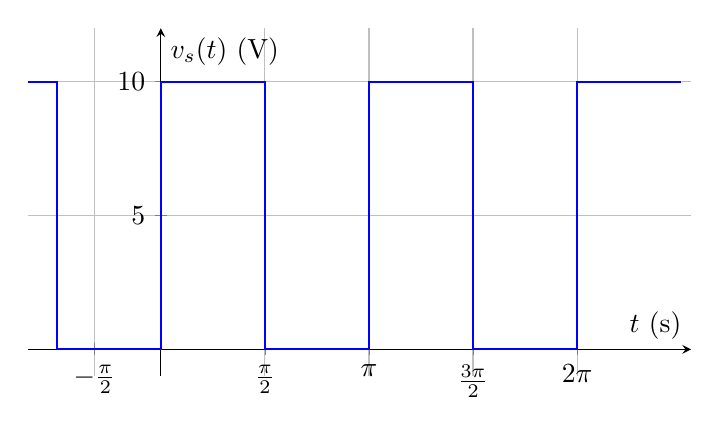
\begin{tikzpicture}
\begin{axis}[
    axis lines = middle,
    xlabel = {$t$ (s)},
    ylabel = {$v_s(t)$ (V)},
    xmin = -2, xmax = 8,
    ymin = -1, ymax = 12,
    xtick = {-1, 0, 1.57, 3.14, 4.71, 6.28},
    xticklabels = {$-\frac{\pi}{2}$, $0$, $\frac{\pi}{2}$, $\pi$, $\frac{3\pi}{2}$, $2\pi$},
    ytick = {0, 5, 10},
    grid = both,
    width=10cm, height=6cm
]
% Period is pi. On for 0 to pi/2, off for pi/2 to pi?
% Need to check the textbook extract vs(t) = 5 + (20/pi) * sum(sin(2nt)/n)
% That Fourier series is for a square wave shifted by 5.
% High at 10, Low at 0. Period is pi.
\addplot[blue, thick, no marks] coordinates {
    (-2, 10)
    (-1.57, 10) (-1.57, 0)
    (0, 0) (0, 10)
    (1.57, 10) (1.57, 0)
    (3.14, 0) (3.14, 10)
    (4.71, 10) (4.71, 0)
    (6.28, 0) (6.28, 10)
    (7.85, 10)
};
\end{axis}
\end{tikzpicture}
\end{document}
